\documentclass[tikz,border=6pt]{standalone}
\usepackage{tikz}
\usetikzlibrary{arrows.meta,bending}
\usepackage{xcolor}

\definecolor{evfill}{RGB}{210,228,250}
\definecolor{evbord}{RGB}{55,95,170}
\definecolor{titlebg}{RGB}{232,241,255}

\newcommand{\ev}[1]{\colorbox{evfill}{\strut\small #1}}

\begin{document}
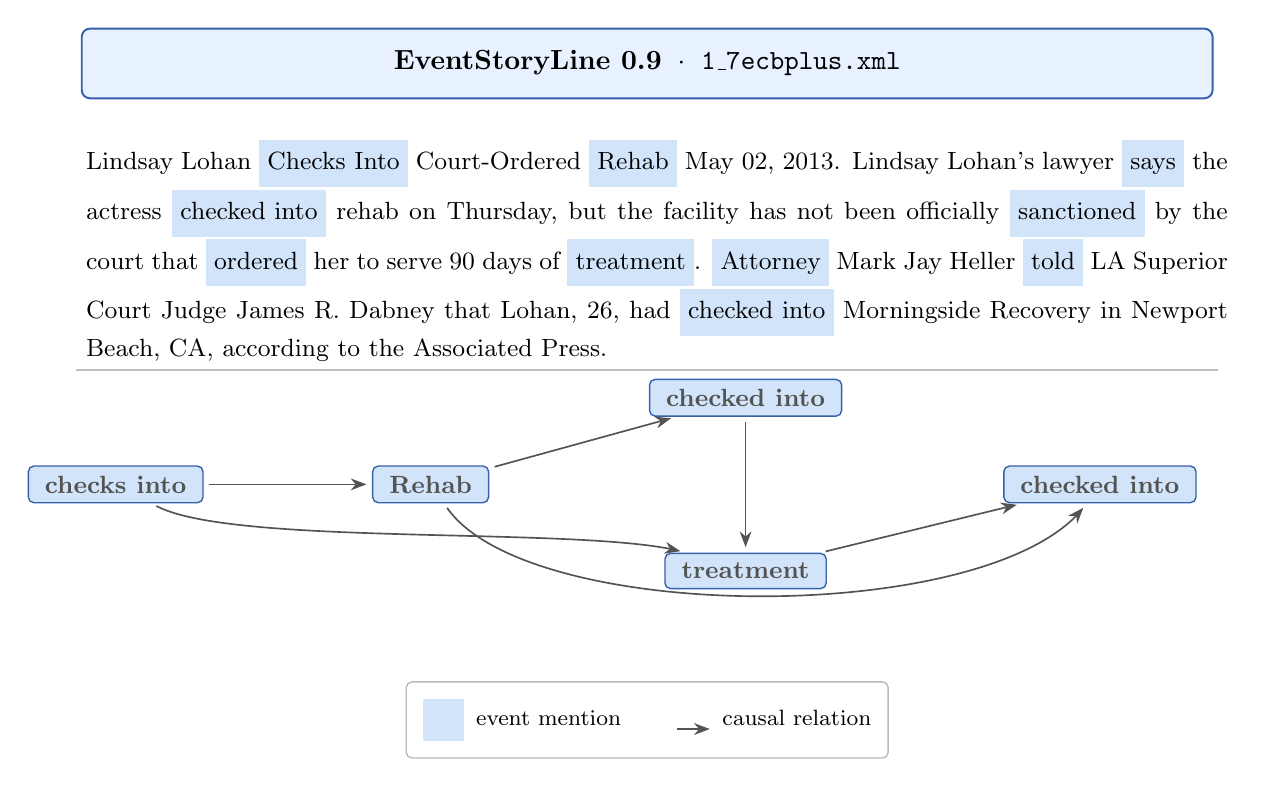
\begin{tikzpicture}[font=\small]

%% ── Title box ────────────────────────────────────────────────────────────────
\node[
  draw=evbord, fill=titlebg, line width=0.7pt,
  rounded corners=3pt, inner sep=8pt,
  anchor=north, text width=13.8cm, align=center,
  font=\normalsize\bfseries
] at (7.25,0) {%
  EventStoryLine~0.9\enspace$\cdot$\enspace\texttt{1\_7ecbplus.xml}%
};

%% ── Annotated text ───────────────────────────────────────────────────────────
\node[anchor=north west, text width=14.5cm, align=justify] at (0,-1.3) {%
Lindsay Lohan \ev{Checks Into} Court-Ordered \ev{Rehab}
May~02, 2013. Lindsay Lohan's lawyer \ev{says} the actress \ev{checked into}
rehab on Thursday, but the facility has not been officially \ev{sanctioned} by
the court that \ev{ordered} her to serve 90~days of \ev{treatment}.
\ev{Attorney} Mark~Jay Heller \ev{told} LA~Superior Court Judge James~R.\
Dabney that Lohan, 26, had \ev{checked into} Morningside Recovery in Newport
Beach, CA, according to the Associated Press.%
};

%% ── Separator ────────────────────────────────────────────────────────────────
\draw[gray!50, line width=0.6pt] (0,-4.35) -- (14.5,-4.35);

%% ── Causal graph ─────────────────────────────────────────────────────────────
\begin{scope}[
  yshift=-5.8cm, xshift=0.5cm,
  every node/.style={
    draw=evbord, fill=evfill, rounded corners=2pt,
    inner xsep=6pt, inner ysep=3.5pt,
    font=\small\bfseries, line width=0.5pt
  },
  -Stealth, semithick, color=gray!65!black,
  shorten >=2pt, shorten <=2pt
]
  \node (n1)  at (0,    0)   {checks into};
  \node (n27) at (4,    0)   {Rehab};
  \node (n2)  at (8,    1.1) {checked into};
  \node (n5)  at (8,   -1.1) {treatment};
  \node (n6)  at (12.5, 0)   {checked into};

  \draw (n1)  -- (n27);
  \draw (n27) -- (n2);
  \draw (n2)  -- (n5);
  \draw (n5)  -- (n6);
  \draw (n27) to[out=-55, in=-125, looseness=0.60] (n6);
  \draw (n1)  to[out=-28, in=163,  looseness=0.45] (n5);
\end{scope}

%% ── Legend box ───────────────────────────────────────────────────────────────
\node[
  draw=gray!55, fill=white, line width=0.5pt,
  rounded corners=2pt, inner sep=6pt,
  anchor=north, font=\footnotesize
] at (7.25,-8.3) {%
  \colorbox{evfill}{\strut\phantom{xx}}\enspace event mention
  \qquad
  \tikz[baseline=0.4ex]{\draw[-Stealth,semithick,gray!65!black](0,0)--(1.4em,0);}\enspace causal relation%
};

\end{tikzpicture}
\end{document}
